% UTF-8

% single-chapter commands
\documentclass[../main/thesis.tex]{subfiles}
\onlyinsubfile{\appendix}  % single-chapter command
\begin{document}



\chapter{Mathematische Konventionen}
\label{appx:mathsymbols}
% zu 4

{\setlength{\doublerulesep}{1mm}%\renewcommand{\arraystretch}{1.1}
\begin{longtable}[c]{|c|p{12cm}|}
\hline
\textbf{Symbol} & \textbf{Beschreibung} \\
\hline
\hline
\endhead
\caption*{(fortgesetzt)}
\endfoot
\caption{Mathematische Abkürzungen und Symbole}
%\label{tab:mathsymbols}
\endlastfoot
\multicolumn{2}{|l|}{\textbf{Bezeichner}} \\
\hline
$\alpha,\beta,\gamma,...$ & Griechische Kleinbuchstaben bezeichnen reelle Größen mit oder ohne Dimension wie Winkel, Längen oder Verhältniszahlen. \\
\hline
$a,b,c,...$ & Lateinische Kleinbuchstaben bezeichnen in aller Regel Vektoren und Segmente. Lediglich solche reelle Größen, für die ein lateinischer Buchstabe im jeweiligen Kontext fest etabliert ist, werden mit lateinischen Buchstaben bezeichnet. \\
\hline
$A,B,C,...$ & Lateinische Großbuchstaben bezeichnen Mengen. \\
\hline
$\mathcal{A},\mathcal{B},\mathcal{C},...$ & Kalligraphische Buchstaben bezeichnen Mengen von Mengen. \\
\hline
\hline
\multicolumn{2}{|l|}{\textbf{Arithmetik und Trigonometrie}} \\
\hline
$\abs[\alpha]$ & absoluter Betrag der Zahl $\alpha$ \\  % Betragsnorm
\hline
$\abs[\mathtowidth[\alpha]{a}]$ & geometrische Länge des Vektors $a$ \\  % euklidische Norm
\hline
$\sphericalangle(a,b)$ & gerichteter rechtsdrehender Winkel von $a$ zu $b$ im Intervall $(-\pi,\pi)$ \\
\hline
\hline
\multicolumn{2}{|l|}{\textbf{Logische Aussagen}} \\
\hline
$\neg$ & nicht \hfill $\neg\,\text{ja} = \text{nein}$ \\
\hline
$\wedge$ & und \\
\hline
$\forall\, M$ & für alle Elemente der Menge $M$ \hfill Allquantor \\
\hline
$\exists\ a$ & es existiert ein Wert für $a$ \hfill Existenzquantor \\
\hline
$\nexists\ a$ & es existiert \emph{kein} Wert für $a$ \\
\hline
$:$ & so dass gilt \\
\hline
\hline
\multicolumn{2}{|l|}{\textbf{Mengen}} \\
\hline
\multicolumn{2}{|p{13cm}|}{Mengen sind ungeordnet und können kein Element mehrfach enthalten.} \\
\hline
$\Set{x \SetCond y}$ & Menge aller $x$, für die Bedingung $y$ gilt \\
\hline
$\Set{a,b}$ & Menge bestehend aus den Elementen $a$ und $b$ \\
\hline
$\TheEmptySet$ & leere Menge \\
\hline
$|M|$ & Anzahl der Elemente der Menge $M$ \\  % Kardinalität
\hline
$\cup$ & Vereinigung \hfill $\Set{a,b} \cup \Set{b,c} = \Set{a,b,c}$ \\
\hline
$\cap$ & Verschneidung \hfill $\Set{a,b} \cap \Set{b,c} = \Set{\mathtowidth[a]{b}}$ \\  % Schnittmenge
\hline
$\setminus$ & Restmenge (gelesen „ohne“) \hfill $\Set{a,b} \setminus \Set{b,c} = \Set{a}$ \\
\hline
$\in$ & Element in Menge \hfill $a \in \Set{a,b}$ \\
\hline
$\subset$ & Teilmenge \hfill $\Set{a} \subset \Set{a,b}$ \\
\hline
\newpage
%\hline
\multicolumn{2}{|l|}{\textbf{Definitionen}} \\
\hline
$a \eqdef b$ & es sei $a$ gleich $b$ \\
\hline
$\rightarrow$ & Definition einer Relation (Assoziation) der genannten Datentypen \\  % mathematisch eigentlich eine aus geordneten Paaren bestehende Klasse
%\hline
%{\small$\eqdefrel$} & Definition des Anfangswerts einer Relation \\
\hline
\myAlgMethodSymbol & Definition eines Algorithmus \\  % identisch mit (d. h. der Name des Algorithmus ist vom Standpunkt des Aufrufers aus austauschbar mit den einzelnen Arbeitsschritten)
\hline
\hline
\multicolumn{2}{|l|}{\textbf{Algorithmen}} \\
\hline
$\textproc{Name}$ & Kurzbezeichnung eines Algorithmus durch dessen Namen \\
\hline
$\triangleright$ & Kommentar \\
\hline
$\hookrightarrow$ & Fortsetzung der vorgehenden Zeile \\
\hline
$\gets$ & Wertzuweisung \\
\hline
$\Nil$ & fehlender Wert (Nullwert) \\  % null pointer / void
\hline
\algorithmicforall & wiederhole die folgenden eingerückten Schritte nacheinander einmal für jedes Element der angegebenen Menge \\
\hline
\algorithmicuntil & wiederhole die eingerückten Schritte nacheinander solange, bis die angegebene Bedingung wahr ist \\
\hline
\algorithmicif & führe die folgenden eingerückten Schritte nur aus genau dann, wenn die angegebene Bedingung wahr ist \\
\hline
\textbf{Ergebnis} & Ergebnis des Algorithmus (Rückgabewert) \\
\hline
\hline
\multicolumn{2}{|l|}{\textbf{Landau-Notation}} \\
\hline
$\mathcal{O}(f)$ & Menge aller Algorithmen, deren Rechenaufwand nicht wesentlich schneller als $f$ wächst \\
\hline
$\hbox{o}(f)$ & Menge aller Algorithmen, deren Rechenaufwand wesentlich langsamer als $f$ wächst \\
\hline
\hline
\multicolumn{2}{|l|}{\textbf{Einheiten und Datentypen}} \\
\hline
px & Pixel \newline die kleinste rechteckige Fläche in gerasterter Darstellung, z.~B. auf dem Bildschirm (für \osm\ in der Regel quadratisch); \newline als Längeneinheit: die Länge einer Pixelreihe von 1\,px Breite \\
\hline
boolean & ja oder nein (bezogen auf die Wahrheit logischer Aussagen) \\
\hline
\end{longtable}
}



\chapter{Bezeichner im Quelltext}
\label{appx:identifiers}
% zu 5.2

\onetable{H}{

\begin{tabular}{|ll|ll|}
\hline
%\multicolumn{2}{|l|}{\textbf{Abschnitt}} & \multicolumn{2}{|l|}{\textbf{Bezeichner im Quelltext}} \\
%\makebox[\widthof{0.0.0}]{$\downarrow$} & \textbf{Bezeichner} & \textbf{Klasse / Interface} & \textbf{Methode} \\
\textbf{In} & \textbf{Bezeichner} & \textbf{Klasse / Interface} & \textbf{Methode} \\
\hline
\ref{ch:split-algorithm} & \textproc{Ende} & \code{\TheJavaPackage Segment} & \code{end} \\
\hline
\ref{ch:split-algorithm} & \textproc{Fußpunkt} & \code{\TheJavaPackage AbstractSegment} & \code{findPerpendicularFoot} \\
\hline
\ref{ch:split-algorithm} & \textproc{Hülle} & \code{\TheJavaPackage SourceSegment} & \code{envelope} \\
\hline
\ref{ch:split-algorithm} & \textproc{NaheSegmente} & \code{\TheJavaPackage Combiner} & \code{regionaliseSegments} \\
% NAHESEGMENTE: Combiner.regionaliseSegments (arbeitet auf SourceSegments, also auf S statt S' und wurzel(s) statt s, weil so die Schnittmengenprüfung nicht wiederholt ausgeführt werden muss und damit ein Spatial Index erleichtert/ermöglicht wird)
\hline
\ref{ch:split-algorithm} & \textproc{Nodes} & \code{\TheJavaPackage NodePair} & \code{other} \\
% NODES: es gibt keine exakte Entsprechung, aber NodePair#other() erfüllt letztlich denselben Zweck, zu dem NODES definiert wurde
\hline
\ref{ch:split-algorithm} & \textproc{Segmente} & \code{\TheJavaPackage highway.Highway} & \code{segmentation} \\
\hline
\ref{ch:split-algorithm} & \textproc{Splitten} & \code{\TheJavaPackage Combiner} & \code{splitSegments} \\
% SPLITTEN: SplitQueueIterator=S' (in Combiner.splitSegments), AbstractLine.splitCloseParallels()=für alle n/t, T enthält schon eine Parallitätsprüfung
\hline
\ref{ch:split-algorithm} & \textproc{Start} & \code{\TheJavaPackage Segment} & \code{start} \\
\hline
\ref{ch:analyse-algorithm} & \textproc{Analyse} & \code{\TheJavaPackage AbstractSegment} & \code{analyse} \\
\hline
\ref{ch:analyse-algorithm} & \textproc{Distanz} & \code{\TheJavaPackage highway.HighwayAnalyser} & \code{distance} \\
\hline
\ref{ch:analyse-algorithm} & \textproc{Mittelpunkt} & \code{\TheJavaPackage NodePair} & \code{midPoint} \\
\hline
\multirow{ 2}{*}{\ref{ch:analyse-algorithm}} & \multirow{ 2}{*}{\textproc{Parallel}} & \code{\TheJavaPackage highway.HighwayAnalyser} & \code{shouldEvaluate} \\
% PARALLEL: SourceSegment.closeParallels / MyAnalyser
 &  & \code{\TheJavaPackage SourceSegment} & \code{closeParallels} \\
\hline
\ref{ch:node-match-algorithm} & \textproc{NodesZuordnen} & \code{\TheJavaPackage NodeGraph} & \code{createGraph} \\
\hline
\ref{ch:generalisation-algorithm} & \textproc{Fortsetzung} & \code{\TheJavaPackage GeneralisedSection} & \code{traverseGraph} \\
\hline
\ref{ch:generalisation-algorithm} & \textproc{Zusammenfassen} & \code{\TheJavaPackage GeneralisedLines} & \code{traverse} \\
\hline
\ref{ch:algorithm-overview} & \textproc{Generalisierung} & \code{\TheJavaPackage Combiner} & \code{run} \\
\hline
\end{tabular}

\caption{Aufschlüsselung der Bezeichner in dieser Arbeit zu denen im Quelltext}
\label{tab:identifiers}
}

Der Quelltext der entwickelten Software ist zusammen mit der zugehörigen API"=Dokumentation zugänglich unter:\\
\url{http://arne.johannessen.de/thesis}




\chapter{Datenmodell und Klassenstruktur}
\label{appx:fullpage-model}
% zu 5.3.2

\onefigure{ht}{
	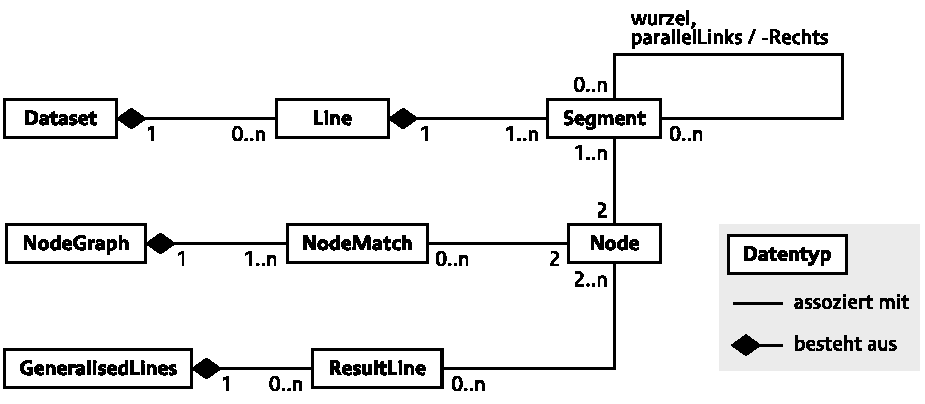
\includegraphics[scale=.77]{../appendices/data-model}
	\caption{Datenmodell}
	\label{fig:appx-data-model}
}

\onefigure{ht!}{
	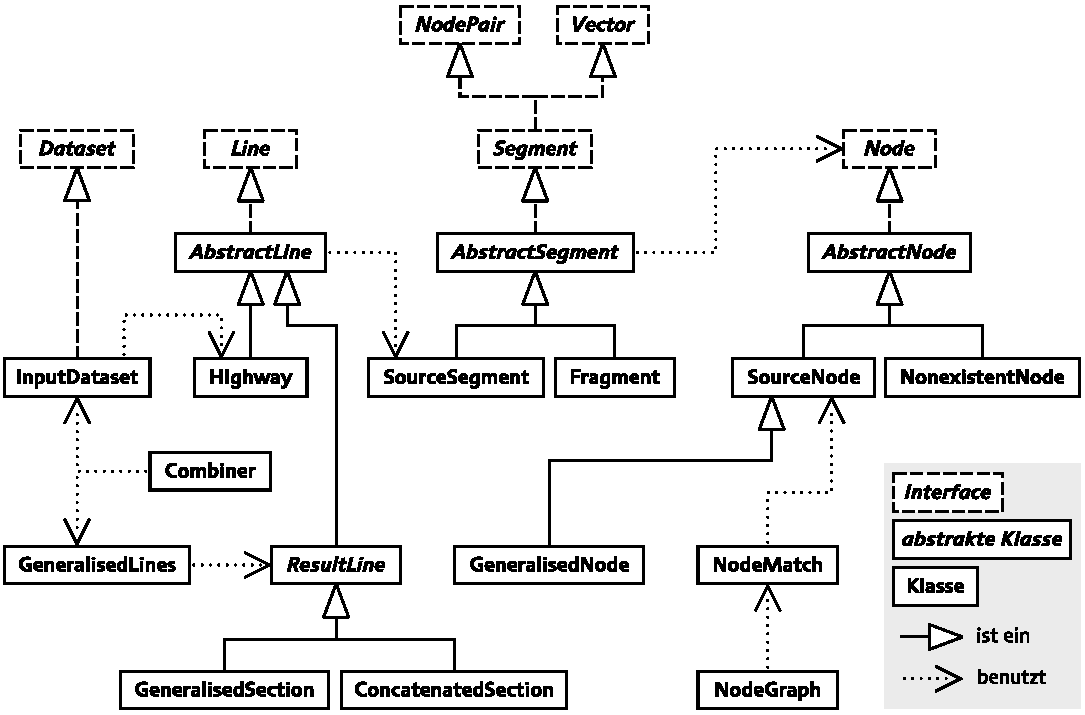
\includegraphics[scale=.77]{../appendices/class-structure}
	\caption
		[Klassenstrukturdiagramm für das Paket \code{comb}]
		{Klassenstrukturdiagramm für das Paket \code{comb} (aus Gründen der Übersichtlichkeit ist nur eine Auswahl der „benutzt“-Beziehungen dargestellt)}
	\label{fig:appx-class-structure}
}



\chapter{Anwendung auf ein Fernstraßennetz}
\label{appx:fullpage-examples-1}
% zu 6
% Beispiel für größeres Gebiet im Zusammenhang in kleinem Maßstab; evtl. unterschiedliche Regionen der Welt
% (Titel könnte sich noch ändern, vgl. E)

TBD



\chapter{Anwendung auf ein innerstädtisches Straßennetz}
\label{appx:fullpage-examples-2}
% zu 6
% Beispiel für größeres Gebiet im Zusammenhang in großem Maßstab; evtl. unterschiedliche Regionen der Welt
% (Titel könnte sich noch ändern, vgl. D)

TBD



\setcounter{chapter}{5}
\chapter{Beispiele für problematische Kreuzungssituationen}
\label{appx:junction-examples}
% zu 6

TBD

~

\noindent
(weitere Beispiele des Scheiterns an unterschiedlichen Kreuzungen; auch zeigen, wie \term{\_links} das Topologielückenproblem hierbei nicht lösen, sondern vergrößern)



%\chapter{Glossar}
%\chapter{Abkürzungsverzeichnis}
%\chapter{Software-Dokumentation}


% single-chapter commands
\end{document}
